\documentclass[11pt,a4paper]{article}
\usepackage[utf8]{inputenc}  % gebruik de juiste 'character encoding'
\usepackage{babel}    % definitie van de taal (Engels is de standaard)
\usepackage{hyperref}        % geef URLs netjes weer
\usepackage{booktabs}		 % mooiere tabellen
\usepackage{a4wide}          % papierformaat en marges
\pagestyle{empty}            % zet paginanummering uit
\usepackage{amsmath,amssymb,amsfonts}
% laad de pakketten voor figuren:
\usepackage{graphicx}
\usepackage{float,flafter}
\usepackage{hyperref}
\usepackage{inputenc}
\usepackage{amssymb}

% titel en auteur van het document
\title{Relativity and Electromagnetism Homework Assignment 4}
\author{Diederik Desmet}
\date{March 2026}
% \date{} % de datum van het document 

% einde definities; start van de tekst
\begin{document}

\maketitle                  % maakt een kopje met titel, auteur en datum
\thispagestyle{empty} 
\section*{Problem 1}
The general solution for the potential is of the form:
\[
V(r,\theta)=\sum^{\infty}_{l=0}\left(A_l r^l + \frac{B_l}{r^{l+1}}\right)P_l(\cos\theta)
\]
analyzing the problem we can immediately see that the potential must of the form:
\[
V(r, \theta)=A_2 r^2 + \frac{B_2}{r^{3}}P_2(\cos\theta) + A_3 r^3 + \frac{B_3}{r^{4}}P_3(\cos\theta)
\]
This is because, at the radius $a$ sphere, the potential must be $V(a, \theta)=V_aP_2(\cos\theta)$, and at the radius $b$ sphere, the potential must be $V(b, \theta)=V_bP_3(\cos\theta)$. there thus has to be a $P_2$ and $P_3$ term, and no other terms.\\
\\
We can now use these boundary conditions to find the coefficients first at the radius $a$ sphere, we find that:
\[
\begin{cases}
A_2 a^2 + \frac{B_2}{a^{3}}=V_a\\
A_3 a^3 + \frac{B_3}{a^{4}}=0
\end{cases}
\]
and at the radius $b$ sphere, we find that:
\[
\begin{cases}
A_2 b^2 + \frac{B_2}{b^{3}}=0\\
A_3 b^3 + \frac{B_3}{b^{4}}=V_b
\end{cases}
\]
combining these two systems of equations we find that:
\[
\begin{cases}
A_2 = \frac{V_a a^3}{a^5 - b^5}\\
B_2 = \frac{V_a a^5 b^3}{b^5 - a^5}\\
\end{cases}
\]
and
\[\begin{cases}
A_3 = \frac{V_b b^4}{b^7 - a^7}\\
B_3 = \frac{V_b b^4 a^7}{a^7 - b^7}
\end{cases}\]
plugging these coefficients back into the general solution we find that the potential in de cavity is given by:
\[
V(r,\theta)=\left(\frac{a^3}{a^5 - b^5}r^2+\frac{a^3b^5}{b^5-a^5}\frac{1}{r^3}\right)V_a P_2(\cos\theta)+\left(\frac{b^4}{b^7 - a^7}r^3+\frac{b^4a^7}{a^7 - b^7}\frac{1}{r^4}\right)V_b P_3(\cos\theta)
\] 
\section*{Problem 2}
for this charge configuration we find that the position vector of the charge at $z=a$, $z=0$ and $z=-a$ are respectively given by:
\[
\left(\begin{matrix}
    0\\0\\a
\end{matrix}\right), \quad
\left(\begin{matrix}
    0\\0\\0
\end{matrix}\right), \quad
\left(\begin{matrix}   
    0\\0\\-a
\end{matrix}\right)
\]

\subsection*{monopole moment}
The monopole moment can be calculated as:
\[
q=\sum_i q_i = 2q - 2q = 0
\]
We thus find that the monopole moment of this charge configuration vanishes.
\subsection*{dipole moment}
The dipole moment can be calculated as:
\[
\mathbf{p}=\sum_i q_i \mathbf{r}_i = 2q\left(\begin{matrix}
    0\\0\\0
\end{matrix}\right) - q\left(\begin{matrix}
    0\\0\\a
\end{matrix}\right) - q\left(\begin{matrix}
    0\\0\\-a
\end{matrix}\right)  = \mathbf{0}
\]
We thus find that the dipole moment of this charge configuration also vanishes.
\subsection*{quadrupole moment}
We can calculate the elements of the quadrupole moment as:
\[
Q_{ij}=\frac{1}{2}\sum_k q_k (3r_{k,i}r_{k,j}-\delta_{ij}r_k^2)
\]
for the diagonal elements we find that:
\[
Q_{xx} = Q_{yy} = qa^2, \quad Q_{zz} = -2qa^2
\]
for the above off-diagonal elements we find that:
\[Q_{xy} = Q_{xz} = Q_{yz} = 0
\]
because the quadrupole moment is symmetric, we find that the quadrupole moment of this charge configuration is given by:
\[\mathbf{Q} = \left(\begin{matrix}
    qa^2 & 0 & 0\\
    0 & qa^2 & 0\\
    0 & 0 & -2qa^2
\end{matrix}\right)
\]
\section*{Problem 3}
\begin{figure}[H]
    \centering
    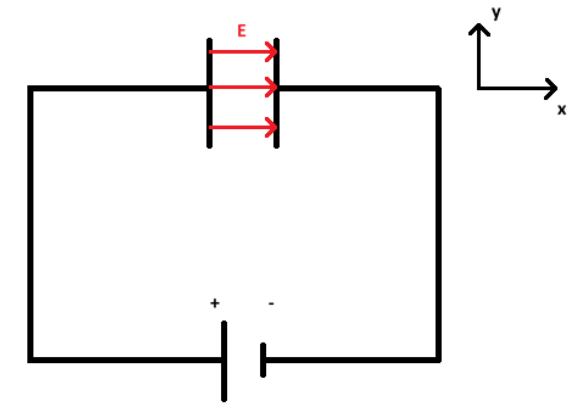
\includegraphics[width=0.5\textwidth]{schakeling.png}
    \caption{Circuit diagram of the problem}
\end{figure}
\subsection*{a.}
\textbf{Electric field}\\
Per definition of the potential difference we have that:
\[
V(d)-V(0)=-\int^d_0 \mathbf{E}\cdot d\mathbf{l}
\]
where $V(0)$ is the potential at the positive plate and $V(d)$ is the potential at the negative plate. Because the electric field is uniform between the plates, we can write that:
\[
V=V(d)-V(0)=-E\int^d_0 dl=-Ed
\] 
Than looking at the circuit, we see that the electric field is pointing in the x-direction and thus we can write that:
\[
\mathbf{E}=-\frac{V}{d}\hat{\mathbf{x}}
\]
\textbf{Polarization}\\
via the relation between the electric field and the polarization:
\[
\mathbf{P}=\epsilon_0(\chi_1+\chi_3E^2)\mathbf{E}
\]
we find that the polarization can be written in terms of the potential as:
\[
\mathbf{P}=-\epsilon_0\left(\chi_1+\chi_3\frac{V^2}{d^2}\right)\frac{V}{d}\hat{\mathbf{x}}
\]   
\textbf{Displacement field}\\
Again via the relation between the electric field, the polarization and the displacement field:
\[
\mathbf{D}=\epsilon_0\mathbf{E}+\mathbf{P}
\]
We find that the displacement field can be written in terms of the potential as:
\[
\mathbf{D}=-\epsilon_0\left(1+\chi_1+\chi_3\frac{V^2}{d^2}\right)\frac{V}{d}\hat{\mathbf{x}}
\]
\subsection*{b.}
\textbf{Free charge}\\
\begin{figure}[H]
    \centering
    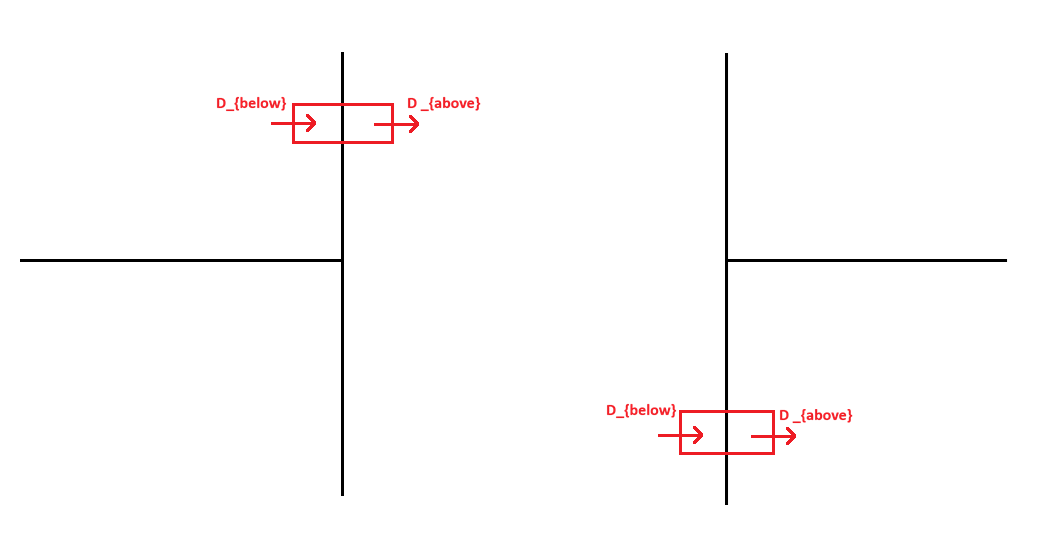
\includegraphics[width=0.6\textwidth]{schakeling2.png}
    \caption{Circuit diagram of the problem with the free charge}
\end{figure}
In the section about boundary conditions (section 4.3.3 edition 4 of Griffiths) we find that the free charge density on the surface of the positive plate can be calculated as:
\[
\sigma_f = D_{above}^{\perp}-D_{below}^{\perp}
\]
for the positive plate, we only have an $D_{above}^{\perp}$ component, becous the electric field is zero outside the plates. We also have that  the displacmentfield is already purpindicular to the surface of the plate, thus we can write that:
\[
\sigma_f(\text{positive plate}) = D_{above}^{\perp}=-\epsilon_0\left(1+\chi_1+\chi_3\frac{V^2}{d^2}\right)\frac{V}{d}
\]
for the negative plate, we only have a $D_{below}^{\perp}$ component, again because the electric field is zero outside the plates. We also have that  the displacmentfield is already purpindicular to the surface of the plate, thus we can write that:
\[
\sigma_f(\text{negative plate}) = -D_{below}^{\perp}=\epsilon_0\left(1+\chi_1+\chi_3\frac{V^2}{d^2}\right)\frac{V}{d}
\]
\textbf{Bound charge}\\
The bounded charge surface density is defined as:
\[
\sigma_b = \mathbf{P}\cdot\hat{\mathbf{n}}
\]
Where $\hat{\mathbf{n}}$ is the normal vector to the surface of the plate, pointing outwards. For the positive plate, we have that $\hat{\mathbf{n}}=\hat{\mathbf{x}}$, thus we can write that:
\[\sigma_b(\text{positive plate}) = \mathbf{P}\cdot\hat{\mathbf{n}}=-\epsilon_0\left(\chi_1+\chi_3\frac{V^2}{d^2}\right)\frac{V}{d}\]
For the negative plate, we have that $\hat{\mathbf{n}}=-\hat{\mathbf{x}}$, thus we can write that:
\[\sigma_b(\text{negative plate}) = \mathbf{P}\cdot\hat{\mathbf{n}}=\epsilon_0\left(\chi_1+\chi_3\frac{V^2}{d^2}\right)\frac{V}{d}\]

\section*{Problem 4}
\subsection*{a.}
because we are working with an diamagnetic sphere, we can expect that the magnetization of the sphere will be in the opposite direction of the external magnetic field. this can also be shown mathematically as folows.
from exercise 6.1 we find that the induced magnetic field inside the sphere $\mathbf{B}_{in}$ from the magnetization is given by:
\[
\mathbf{B}_{induced} = \frac{3}{2}\epsilon_0 \mathbf{M}
\]
so that the total magnetic field inside the sphere is given by:
\[
\mathbf{B}_{tot} = \mathbf{B}_0 + \mathbf{B}_{induced} = B_0\hat{\mathbf{z}} + \frac{3}{2}\epsilon_0 \mathbf{M}
\]
we also have that the total magnetic field inside the sphere is given by:
\[
\mathbf{B}_{tot} = \mu_0(\mathbf{H}_{in}+\mathbf{M})
\]
and that the magnetization is related to the H-field via the relation:
\[
\mathbf{M} = \chi_m \mathbf{H}_{in}
\]
combining these three equations we find that:
\[
\frac{1}{\chi_m}\mathbf{M}=\frac{B_0}{\mu_0}\hat{\mathbf{z}} -\frac{1}{3}\mathbf{M} \quad \Leftrightarrow \quad \boxed{\mathbf{M} = -\frac{B_0}{\mu_0}\left(\frac{3|\chi_m|}{3-|\chi_m|}\right)\hat{\mathbf{z}}}
\]
And because $\chi_m$ is negative for a diamagnetic material, we find that the magnetization of the sphere is indeed in the opposite direction of the external magnetic field. the total magnetic field inside the sphere can then be calculated as:

\[
\boxed{
\mathbf{B}_{in} = \frac{3-3|\chi_m|}{3-|\chi_m|}B_0\hat{\mathbf{z}}
}
\]
For the magnetic field outside the sphere, we can use the fact that the magnetization of the sphere is equivalent to a magnetic dipole moment $\mathbf{m}$ located at the center of the sphere, with $\mathbf{m} = \frac{4}{3}\pi R^3 \mathbf{M}$ where $R$ is the radius of the sphere. The magnetic field outside the sphere can then be calculated using the formula for the magnetic field of a dipole:
\begin{align*}
\mathbf{B}_{dip} &= \frac{\mu_0}{4\pi r^3}\left(2\cos\theta\hat{\mathbf{r}} + \sin\theta\hat{\mathbf{\theta}}\right)\cdot \mathbf{m}\\
&= \frac{\mu_0}{4\pi r^3}\left(2\cos\theta\hat{\mathbf{r}} + \sin\theta\hat{\mathbf{\theta}}\right)\cdot \frac{4}{3}\pi R^3 \mathbf{M}\\
&= \frac{\mu_0 R^3}{3 r^3}\left(2\cos\theta\hat{\mathbf{r}} + \sin\theta\hat{\mathbf{\theta}}\right)\cdot \mathbf{M}
\end{align*}

and we thus find that the total magnetic field outside the sphere is given by:
\[
\boxed{
\mathbf{B}_{out} = \mathbf{B}_0 + \mathbf{B}_{dip} = B_0\hat{\mathbf{z}} + \frac{\mu_0 R^3}{3 r^3}\left(2\cos\theta\hat{\mathbf{r}} + \sin\theta\hat{\mathbf{\theta}}\right)\cdot \mathbf{M}
}
\]
using the urlier relations we can calculate the H-field inside and outside the sphere respectively as:
\[\boxed{\mathbf{H}_{in} = \frac{3}{3-|\chi_m|}\frac{B_0}{\mu_0}\hat{\mathbf{z}}} \quad \boxed{\mathbf{H}_{out} = \frac{B_0}{\mu_0}\hat{\mathbf{z}} + \frac{R^3}{3 r^3}\left(2\cos\theta\hat{\mathbf{r}} + \sin\theta\hat{\mathbf{\theta}}\right)\cdot \mathbf{M}}
\]
These fields can be scatched as follows:

\begin{figure}[H]
    \centering
    \begin{minipage}{0.3\textwidth}
        \centering
        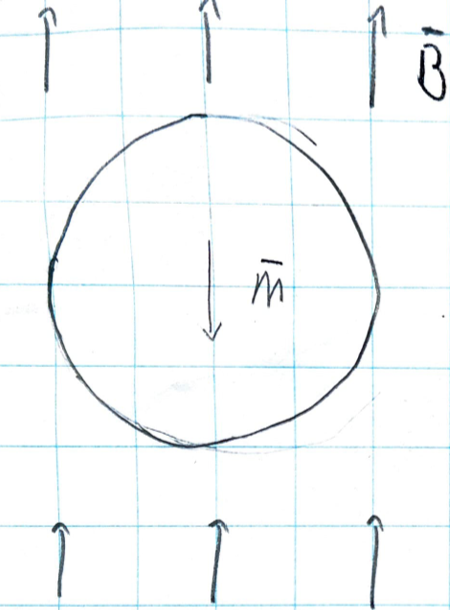
\includegraphics[width=\textwidth]{magnetisatie.png}
        \caption{the magnetization of the sphere}
    \end{minipage}\hfill
    \begin{minipage}{0.3\textwidth}
        \centering
        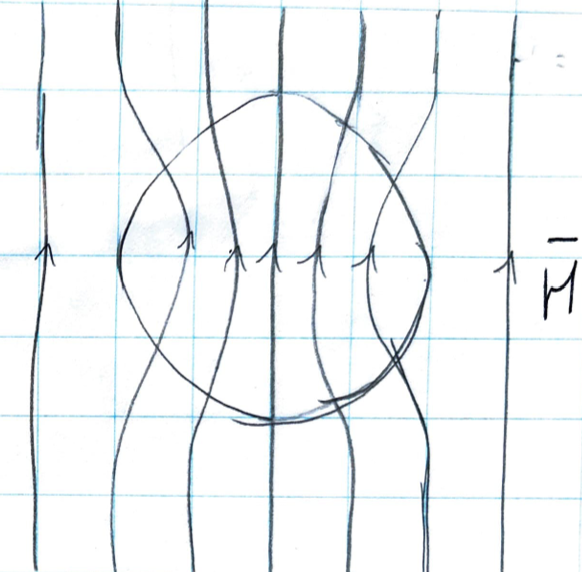
\includegraphics[width=\textwidth]{H-veld.png}
        \caption{the H-field}
    \end{minipage}\hfill
    \begin{minipage}{0.3\textwidth}
        \centering
        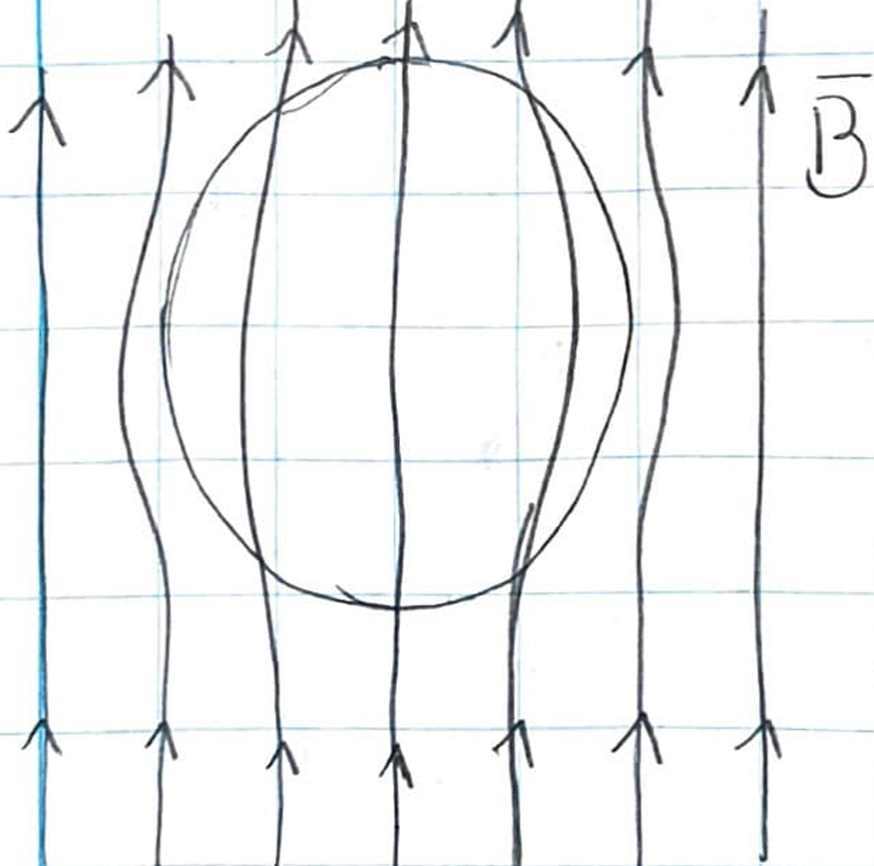
\includegraphics[width=\textwidth]{magnetisch-veld.png}
        \caption{the magnetic field}
    \end{minipage}
\end{figure}
\subsection*{b.}
The induced surface current density on the sphere can be calculated as:
\[\mathbf{K} = \mathbf{M}\times\hat{\mathbf{n}} \]
where $\hat{\mathbf{n}}$ is the normal vector to the surface of the sphere, pointing outwards. Because we are working with a sphere, we have that $\hat{\mathbf{n}}=\hat{\mathbf{r}}$ and $\hat{\mathbf{z}}=\hat{\mathbf{r}}\cos\theta-\hat{\mathbf{\theta}}\sin\theta$ so that we can write that:
\[\mathbf{K} = -\frac{B_0}{\mu_0}\left(\frac{3|\chi_m|}{3-|\chi_m|}\right)\hat{\mathbf{z}}\times\hat{\mathbf{r}} = -\frac{B_0}{\mu_0}\left(\frac{3|\chi_m|}{3-|\chi_m|}\right)\hat{\mathbf{\phi}}\sin\theta
\]
\section*{Problem 5}
\subsection*{a.}
using the hint given in the problem, we first calculate the elektric field within the overlap region of the two spheres. the electric field within a sphere with a uniform charge distribution can be calculated using Gauss's law as:
\[\mathbf{E} = \frac{1}{4\pi\epsilon_0}\frac{Q}{R^3}\mathbf{r}\]
where $Q$ is the total charge of the sphere, $R$ is the radius of the sphere and $\mathbf{r}$ is the position vector from the center of the sphere. we set our coordinate system such that the center of the positive sphere is at $(0,\frac{d}{2})$ and the center of the negative sphere is at $(0,-\frac{d}{2})$. thus the electric field of the positive and negative sphere becomes respectively:
\[\mathbf{E}_{positive} = \frac{1}{4\pi\epsilon_0}\left(\frac{\mathbf{r}-\frac{d}{2}\hat{\mathbf{z}}}{R^3}\right)\]
\[\mathbf{E}_{negative} = -\frac{1}{4\pi\epsilon_0}\left(\frac{\mathbf{r}+\frac{d}{2}\hat{\mathbf{z}}}{R^3}\right)\]
using than the principle of superposition we can calculate the total electric field in the overlap region as:   
\begin{align*}
\mathbf{E} &= \mathbf{E}_{positive} + \mathbf{E}_{negative}\\
&= \frac{1}{4\pi\epsilon_0}\left(\frac{\mathbf{r}-\frac{d}{2}\hat{\mathbf{z}}}{R^3}\right) - \frac{1}{4\pi\epsilon_0}\left(\frac{\mathbf{r}+\frac{d}{2}\hat{\mathbf{z}}}{R^3}\right)\\
&= \frac{1}{4\pi\epsilon_0}\frac{Qd}{R^3}\hat{\mathbf{z}}\\
&= \frac{1}{4\pi\epsilon_0}\frac{\mathbf{d}}{R^3}
\end{align*}
then using the hint given in the problem, we fill in the polarization of the spheres as $\mathbf{p} = \frac{4}{3}\pi R^3\mathbf{P}$  and so find the relation we where lookinf for:
\[\mathbf{E} = -\frac{1}{3\epsilon_0}\mathbf{P}\]
\subsection*{b.}
from the relation $\mathbf{E}=\mathbf{E}_{ext}+\mathbf{E}_{self}$, and using $\mathbf{E}=\frac{1}{\chi_e \epsilon_0}\mathbf{P}$, $\mathbf{E}_{ext}=\frac{1}{N\alpha}\mathbf{P}$ and the above relation for $\mathbf{E}_{self}$ we find that:
\[
\frac{1}{\chi_e \epsilon_0}\mathbf{P} = \frac{1}{N\alpha} - \frac{1}{3\epsilon_0}\mathbf{P}
\quad \Leftrightarrow \quad \frac{1}{\chi_e \epsilon_0} = \frac{1}{N\alpha} - \frac{1}{3\epsilon_0}
\quad \Leftrightarrow \quad \boxed{\chi_e = \frac{3N\alpha}{3\epsilon_0 - N\alpha}}
\]
\section*{Problem 6}
\subsection*{a.}
beacous we are interested in de radiation field, which is the field at large distances from the source, we can use the approximation $r >> \frac{\omega}{c}$ witch only leaves the first term of the potential of the oscilating magnetic dipole:
\[\mathbf{A}(\mathbf{r}, t) \approx -\frac{\mu_0m_0\omega\sin\theta}{4\pi c r}sin[\omega(t-\frac{r}{c})]\]
we can thus conclude that it is the first term of the potential that dominates the radiation field.
\subsection*{b.}
because the scalar potential vanishes, we have that the electric- and magnetic field can be calculated respectively as:
\[\mathbf{E}=-\frac{\partial \mathbf{A}}{\partial t} \quad \mathbf{B}=\nabla\times\mathbf{A}\]
plugging in the given vector potential we find for the electric field:
\begin{align*}
\mathbf{E} &= -\frac{\partial \mathbf{A}}{\partial t}\\
&= -\frac{\mu_0 m_0 \sin\theta}{4\pi r}\left(-\frac{\omega^2}{c} \cos[\omega(t-\frac{r}{c})]-\frac{\omega}{r}\sin[\omega(t-\frac{r}{c})]\right)\hat{\mathbf{\phi}}
\end{align*}
and for the magnetic field we find that:
\begin{align*}
\mathbf{B} &= \nabla\times\mathbf{A}\\
&= \frac{1}{r\sin\theta}\frac{\partial}{\partial\theta}(A_{\phi}\sin\theta)\hat{\mathbf{r}}-\frac{1}{r}\frac{\partial}{\partial r}(rA_{\phi})\hat{\mathbf{\theta}}\\
&= \frac{1}{r\sin\theta}\left(\frac{\sin(2\theta)}{\sin\theta}A_{\phi}\right)\hat{\mathbf{r}}-\frac{\mu_0m_0\sin\theta}{4\pi r}\left[\left(\frac{\omega}{c}\right)^2\cos(\omega(t-\frac{r}{c}))-\frac{1}{r^2}\cos(\omega(t-\frac{r}{c}))+\frac{\omega}{rc}\sin(\omega(t-\frac{r}{c}))\right]\hat{\mathbf{\theta}}
\end{align*}
And again making the approximation that $r >> \frac{\omega}{c}$ so that $\frac{1}{r^2}\approx 0$ we find that the electric and magnetic field in the radiation zone can be approximated as:
\[\mathbf{E} \approx \frac{\mu_0 m_0 \omega^2}{4\pi c }\left(\frac{\sin\theta}{r}\right) \cos[\omega(t-\frac{r}{c})]\hat{\mathbf{\phi}}\]
\[ \mathbf{B} \approx -\frac{\mu_0 m_0 \omega^2}{4\pi c^2 }\left(\frac{\sin\theta}{r}\right) \cos[\omega(t-\frac{r}{c})]\hat{\mathbf{\theta}}\]   
\subsection*{c.}
the Poynting vector is deffined as:
\[
\mathbf{S} = \frac{1}{\mu_0}\mathbf{E}\times\mathbf{B}
\]
plugging in the approximated electric and magnetic field we find:
\begin{align*}
\mathbf{S} &= \frac{1}{\mu_0}\mathbf{E}\times\mathbf{B}\\
&= \frac{1}{\mu_0}\frac{\mu_0^2 m_0^2 \omega^4}{16\pi^2 c^3 }\left(\frac{\sin^2\theta}{r^2}\right) \cos^2[\omega(t-\frac{r}{c})]\hat{\mathbf{r}}\\
&= \frac{\mu_0 m_0^2 \omega^4}{16\pi^2 c^3 }\left(\frac{\sin^2\theta}{r^2}\right) \cos^2[\omega(t-\frac{r}{c})]\hat{\mathbf{r}}
\end{align*}
we see that the Poynting vector is pointing in the radial direction. the intensity of the radiation can be calculated as the time average of the magnitude of the Poynting vector:
\begin{align*}
    \langle \mathbf{S} \rangle &= \frac{\mu_0 m_0^2 \omega^4}{16\pi^2 c^3 }\left(\frac{\sin^2\theta}{r^2}\right) \langle\cos^2[\omega(t-\frac{r}{c})]\rangle\hat{\mathbf{r}}\\
    &= \frac{\mu_0 m_0^2 \omega^4}{16\pi^2 c^3 }\left(\frac{\sin^2\theta}{r^2}\right) \frac{1}{2}\hat{\mathbf{r}}\\
    &= \frac{\mu_0 m_0^2 \omega^4}{32\pi^2 c^3 }\left(\frac{\sin^2\theta}{r^2}\right)\hat{\mathbf{r}}
\end{align*}
and thus we find that the intensity of the radiation is given by:
\end{document}